\section{S\&P500 Prices}
Our equity price dataset consists of daily closing prices of S\&P500 downloaded from Federal Reserve Economic Data (FRED of St. Louis Fed, 2021). These closing prices are updated only on trading days in the U.S. stock market, i.e., they are updated only on weekdays. Moreover, closing prices for some weekdays are also unavailable due to stock market holidays. During the investigated time period between February 28, 2020 and October 5, 2020, there were 4 weekdays worth of stock market holidays, when S\&P500 trading was halted (i.e.,. 10 April 2020; 25 May 2020; 3 July, 2020; and 7 September 2020. Data for these days are, therefore, unavailable. 

\begin{figure}[htp]
    \centering
    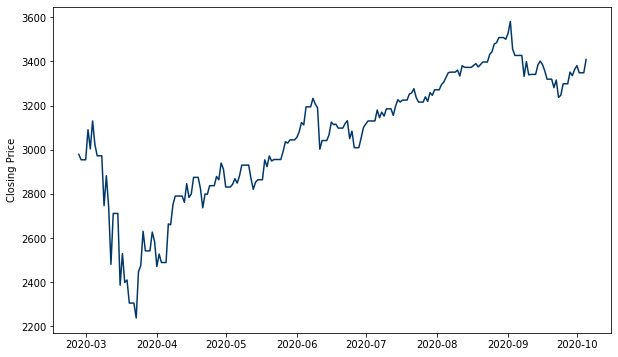
\includegraphics[width=12cm]{methods/ClosingPrice.png}
    \caption{Daily closing price of S\&P500 index.}
    \label{fig:ClosingPrice}
\end{figure}

The missing S&P500 prices for weekends and stock market holidays can be addressed either by (a) using linear interpolation to fill in the time series gaps, as in \textcite{davis2021stock} or by (b) excluding these days entirely from analysis, as in \textcite{bollen2011twitter}. We exclude the days from analysis to prevent potential bias that interpolation could introduce. Nonetheless, to be able to link S&P500 prices to the Twitter data, we must also exclude the same days from the Twitter dataset.
